\documentclass[]{article}

\usepackage{booktabs} % For \toprule, \midrule and \bottomrule
\usepackage{pgfplotstable} % Generates table from .csv
\usepackage{siunitx} % Formats the units and values
\usepackage{graphicx}
\usepackage{amsmath}

%opening
\title{\Huge ME6406 HW3\\Thanakorn Khamvilai}
\author{}
\date{}

% Setup siunitx:
\sisetup{
	round-mode          = places, % Rounds numbers
	round-precision     = 4, % to 4 places
}

\begin{document}

\pagenumbering{gobble}
\maketitle
\newpage
\pagenumbering{arabic}

\section{Camera Model and Calibration}
\subsection{a) Camera Model}
CameraCalibration.m\\
\\
\indent The 2D image coordinates are shown in Table \ref{tab:table1}

\begin{table}[h!]
	\centering
	\caption{2D image coordinates (uv)}
	\label{tab:table1}
	\pgfplotstabletypeset[
		multicolumn names, % allows to have multicolumn names
		col sep=comma, % the seperator in our .csv file
		display columns/0/.style={
			column name=$u\ coordinate$, % name of first column
			column type={S},string type},  % use siunitx for formatting
		display columns/1/.style={
			column name=$v\ coordinate$,
			column type={|S},string type},
		every head row/.style={
			before row={\toprule}, % have a rule at top
			after row={
		%		\si{\ampere} & \si{\volt}\\ % the units seperated by &
				\midrule} % rule under units
		},
		every last row/.style={after row=\bottomrule}, % rule at bottom
		]{camera_calibration_data.csv} % filename/path to file
\end{table}

\indent and the plots are illustrated in Fig \ref{fig:fig1}

\newpage
\begin{figure}[h!]
	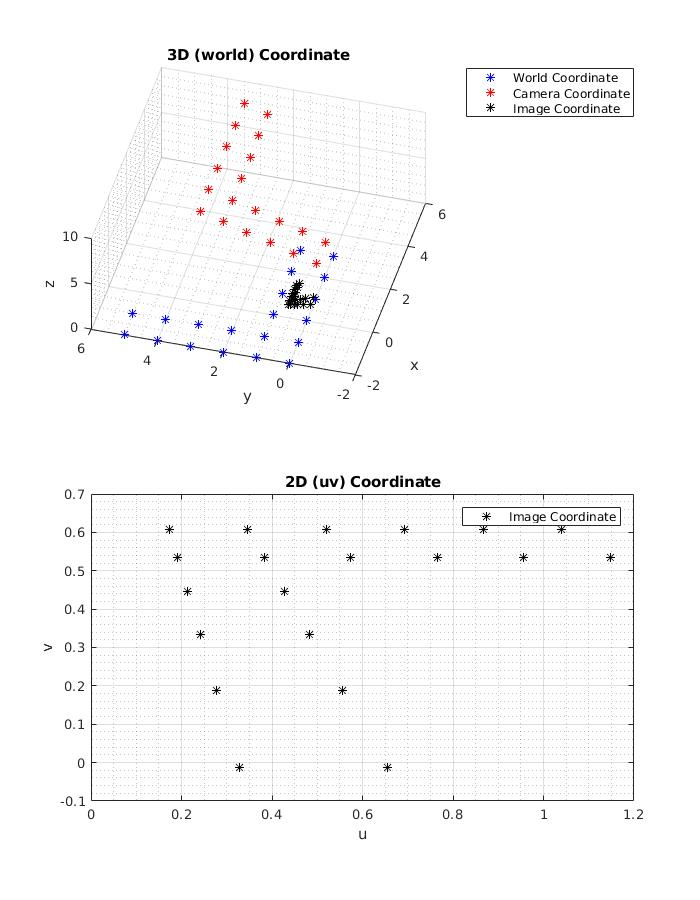
\includegraphics[width=\linewidth]{1a.jpg}
	\caption{Camera model and calibration}
	\label{fig:fig1}
\end{figure}

\newpage
\subsection{b) Camera Calibration}
CameraModel.m\\
\\
Step 1) load 'camera\_calibration\_data.mat' and construct $[\textbf{A}]$, and $\textbf{b}$
\begin{align*}
A &=
\begin{bmatrix}
X_1v_{d1} & Y_1v_{d1} & -X_1u_{d1} & -Y_1u_{d1} & v_{d1}\\
 & & . & &\\
 & & . & &\\
 & & . & &\\
X_nv_{dn} & Y_nv_{dn} & -X_nu_{dn} & -Y_nu_{dn} & v_{dn}\\
\end{bmatrix}\\
\\
b &=
\begin{bmatrix}
u_{d1}\\
.\\
.\\
.\\
u_{dn}
\end{bmatrix}\\
\\
A\mu &= b
\end{align*}
\indent where $\mu$ can be solved using Pseudo-Inverse method and defined by
\begin{align*}
\mu &=
\begin{bmatrix}
r_{11}/T_y\\
r_{12}/T_y\\
r_{21}/T_y\\
r_{22}/T_y\\
T_x/T_y
\end{bmatrix}\\
\end{align*}
\indent Note that $r_{ij}$ is the element of $[\textbf{R}]$, and $T_x$, $T_y$ are the x, and y element of $\textbf{T}$, respectively\\
\\
\indent With the loaded data
\newpage
\begin{align*}
A &=
\begin{bmatrix}
 -1.2133 &        0 &   0.3467 &        0 &   0.6067\\
-0.6067  &       0 &   0.3467  &       0 &   0.6067\\
0   &      0    &     0     &    0 &   0.6067\\
0.6067    &     0  & -0.6933    &     0 &   0.6067\\
1.2133     &    0 &  -1.7333     &    0 &   0.6067\\
1.8200    &     0 &  -3.1200     &    0 &   0.6067\\
-1.0690 &   0.5345  &  0.3828 &  -0.1914 &   0.5345\\
-0.5345  &  0.5345  &  0.3828 &  -0.3828  &  0.5345\\
0  &  0.5345     &    0  & -0.5741   & 0.5345\\
0.5345  &  0.5345 &  -0.7655  & -0.7655  &  0.5345\\
1.0690  &  0.5345 &  -1.9138  & -0.9569  &  0.5345\\
1.6035 &   0.5345&   -3.4448 &  -1.1483  &  0.5345\\
-0.4456 &   0.8911 &   0.4272 &  -0.8544 &   0.4456\\
-0.8911 &   0.8911 &   0.4272 &  -0.4272  &  0.4456\\
-0.3332  &  0.9997 &   0.4834 &  -1.4502  &  0.3332\\
-0.6664  &  0.9997 &   0.4834 &  -0.7251  &  0.3332\\
-0.1869 &   0.7475  &  0.5566 &  -2.2262 &   0.1869\\
-0.3738 &   0.7475 &   0.5566 &  -1.1131  &  0.1869\\
0.0117 &  -0.0583  &  0.6558  & -3.2791 &  -0.0117\\
0.0233 &  -0.0583 &   0.6558 &  -1.6396 &  -0.0117
\end{bmatrix}\\
\\
b &=
\begin{bmatrix}
0.1733\\
0.3467\\
0.5200\\
0.6933\\
0.8667\\
1.0400\\
0.1914\\
0.3828\\
0.5741\\
0.7655\\
0.9569\\
1.1483\\
0.4272\\
0.2136\\
0.4834\\
0.2417\\
0.5566\\
0.2783\\
0.6558\\
0.3279
\end{bmatrix}\\
\end{align*}
\indent Therefore, $\mu$ is
\begin{align*}
 \mu &=
 \begin{bmatrix}
 \mu_1\\
 \mu_2\\
 \mu_3\\
 \mu_4\\
 \mu_5
 \end{bmatrix} =
 \begin{bmatrix}
 	0.2857\\
 	0.0000\\
 	0.0000\\
 	-0.2020\\
 	0.8571
 \end{bmatrix}\\
\end{align*}
\indent Since, $\mu_1\mu_4 \neq \mu_2\mu_3, then \ T_y^2$ can be calculated from\\
\begin{align*}
T_y^2 &= \frac{U-[U^2-4(\mu_1\mu_4-\mu_2\mu_3)^2]^{1/2}}{2(\mu_1\mu_4-\mu_2\mu_3)^2}
\end{align*}
\indent where
\begin{align*}
U &= \sum_{j=1}^{4}\mu_j^2
\end{align*}
\indent Therefore,
\begin{align*}
T_y &= 12.25
\end{align*}
\indent Then each element of $[\textbf{R}]$ can be determined
\begin{align*}
r_{ij} &= \mu_{ij}T_y \ (i,j = 1,2)\\
r_{13}^2 &= 1-T_y^2(\mu_1^2+\mu_2^2)\\
r_{23}^2 &= 1-T_y^2(\mu_3^2+\mu_4^2)\\
\begin{bmatrix}
r_{31}\\
r_{32}\\
r_{33}
\end{bmatrix} &=
\begin{bmatrix}
r_{11}\\
r_{12}\\
r_{13}
\end{bmatrix} \times
\begin{bmatrix}
r_{21}\\
r_{22}\\
r_{23}
\end{bmatrix}
\end{align*}
\indent There is a step to check the sign of $T_y$; however, in this problem the sign of $T_y$ is already correct (positive).\\
\\\
\indent Since, the sign of $r_{11}r_{21}+r_{12}r{22}]$ is not negative, the sign of $r_{23}$ must be flipped.\\
\\
\indent The matrix $[\textbf{R}]$, and the vector $\textbf{T}$ can be constructed as
\begin{align*}
R &=
\begin{bmatrix}
1 & 0 & 0\\
0 & -0.7071 & 0.7071\\
0 & -0.7071 & -0.7071
\end{bmatrix}\\
\\
T &=
\begin{bmatrix}
3.0\\
3.5\\
T_z
\end{bmatrix}\\
\end{align*}

\newpage
Step 2) Construct $[\textbf{A'}], \textbf{x'}$, and $\textbf{b'}$ in the similar way as  $[\textbf{A}], \mu,$ and $\textbf{b}$
\begin{align*}
A'x' &= b'
\end{align*}
where
\begin{align*}
A' &=
\begin{bmatrix}
x_1 & r_{d1}^2x_1 & -u_{d1}\\
& . &\\
& . & \\
& . & \\
x_n & r_{dn}^2x_n & -u_{dn}\\
\end{bmatrix}\\
\\
x' &=
\begin{bmatrix}
f\\
fk_1\\
T_z\\
\end{bmatrix}\\
\\
b' &= 
\begin{bmatrix}
(r_{31}X_1+r_{32}Y_1)u_{d1}\\
.\\
.\\
.\\
(r_{31}X_n+r_{32}Y_n)u_{dn}
\end{bmatrix}\\
\\
x_i &= r_{11}X_i+r_{12}Y_i+T_x
\end{align*}
\indent Therefore, $x'$ can be calculated from Pseudo-Inverse Method
\begin{align*}
x' &=
\begin{bmatrix}
1.3\\
0\\
7.5\\
\end{bmatrix}
\end{align*}
\indent Hence, the value of $f, [\textbf{R}], \textbf{T}$ is computed and shown in the following equations.\\	
\begin{align*}
f &= 1.3\\
\\
R &=
\begin{bmatrix}
1 & 0 & 0\\
0 & -0.7071 & 0.7071\\
0 & -0.7071 & -0.7071
\end{bmatrix}\\
\\
T &=
\begin{bmatrix}
3.0\\
3.5\\
7.5
\end{bmatrix}\\
\end{align*}

\newpage
\section{Robot Eye-on-Hand Calibration}
\subsection{Compute ([Rc12], Tc12) and ([Rc23], Tc23)}
HW3\_2.m\\
\\
\indent Since $H_{c1}$, $H_{c2}$, and $H_{c3}$ are given, $H_{c12}$, and $H_{c23}$ can be calculated from the following equation.
\begin{align*}
H_{cij} &= H_{cj}H_{ci}^{-1}
\end{align*}

\indent  Then, $R_{c12}, T_{c12}, R_{c23},$ and $T_{c23}$ can be extracted from $H_{c12}$, and $H_{c23}$ using the following equation.
\begin{align*}
H_{ij} &=
\begin{bmatrix}
 & R_{ij} & & T_{ij}\\
0 & 0 & 0 & 1
\end{bmatrix}
\end{align*}

\indent Therefore, $R_{c12}, T_{c12}, R_{g23},$ and $T_{g23}$ are
\begin{align*}
R_{c12} &=
\begin{bmatrix}
-0.0718 &  0.8417 & -0.5351 \\
-0.7548 & -0.3965 & -0.5225 \\
-0.6520 &  0.3664 &  0.6638 \\
\end{bmatrix}\\
\\
T_{c12} &=
\begin{bmatrix}
0.1319\\
5.2006\\
-2.8082\\
\end{bmatrix}\\
\\
R_{c23} &=
\begin{bmatrix}
-0.1863 & -0.0898 &  0.9784\\
0.4973  &  0.8502 &  0.1727\\
-0.8473 &  0.5187 & -0.1138\\
\end{bmatrix}\\
\\
T_{c23} &=
\begin{bmatrix}
-4.3792\\
-1.2780\\
5.4939\\
\end{bmatrix}
\end{align*}

\newpage
\subsection{Obtain the equivalent angle-axis representation ($n, \theta$) for each of the rotation matrices; [Rc12], [Rc23], [Rg12] and [Rg23].}
HW3\_2.m\\
\\
\indent Since $H_{g12}$, and $H_{g23}$ are given, $R_{g12}$, $T_{g12}$, $R_{g23}$, and $T_{g23}$ can be extracted in the same way as in 2.1.\\
\\
\indent $(n, \theta)$ can be calculated from the following equations.
\begin{align*}
\theta &= arccos
\left(
\frac{R_{11}+R_{22}+R_{33}-1}{2}
\right)\\
n &= \frac{sin(\theta)}{2}
\begin{bmatrix}
R_{32}-R_{23}\\
R_{13}-R_{31}\\
R_{21}-R_{12}\\
\end{bmatrix}
\end{align*}

\indent Note that
\begin{align*}
R &= 
\begin{bmatrix}
R_{11} & R_{12} & R_{13} \\
R_{21} & R_{22} & R_{23} \\
R_{31} & R_{32} & R_{33} \\
\end{bmatrix}
\end{align*}

\indent Therefore, $(n, \theta)$ for each of the rotation matrices are
\begin{align*}
n_{c12} &=
\begin{bmatrix}
0.4855\\
0.0639\\
-0.8719\\
\end{bmatrix}\\
\theta_{c12} &= 113.7181\\
n_{c23} &=
\begin{bmatrix}
0.1776\\
0.9369\\
0.3013\\
\end{bmatrix}\\
\theta_{c23} &= 102.9986\\
n_{g12} &=
\begin{bmatrix}
-0.0639\\
0.4856\\
-0.8718\\
\end{bmatrix}\\
\theta_{g12} &= 113.7127\\
n_{g23} &=
\begin{bmatrix}
-0.9369\\
0.1773\\
0.3014\\
\end{bmatrix}\\
\theta_{g23} &= 102.9843\\
\end{align*}

\newpage
\subsection{Compute Pc12, Pc23, Pg12, and Pg23.\\ Check the solutions}
HW3\_2.m\\
\\
\indent P can be calculated from $(n, \theta)$ using the following equation.
\begin{align*}
P &= 2sin\left(\frac{\theta}{2}\right)n
\end{align*}
\indent Therefore, $P_{c12}, P_{c23}, P_{g12},$ and $P_{g23}$ are
\begin{align*}
P_{c12} &=
\begin{bmatrix}
0.8130\\
0.1069\\
-1.4602\\
\end{bmatrix}\\
P_{c23} &=
\begin{bmatrix}
0.2779\\
1.4664\\
0.4715\\
\end{bmatrix}\\
P_{g12} &=
\begin{bmatrix}
-0.1070\\
0.8132\\
-1.4600\\
\end{bmatrix}\\
P_{g23} &=
\begin{bmatrix}
-1.4663\\
0.2774\\
0.4716\\
\end{bmatrix}
\end{align*}
\indent To check the solution R can be backwardly calculated from $(n,\theta)$ and P from the following equations.
\begin{align*}
R &= 
\begin{bmatrix}
n_1^2 + (1-n_1^2)cos(\theta) & n_1n_2(1-cos(\theta))-n_3sin(\theta) & n_1n_3(1-cos(\theta))+n_2sin(\theta) \\
n_1n_2(1-cos(\theta))+n_3sin(\theta)   & n_2^2+(1-n_2^2)cos(\theta)  & n_2n_3(1-cos(\theta))-n_1sin(\theta) \\
n_1n_3(1-cos(\theta))-n_2sin(\theta)   & n_2n_3(1-cos(\theta))+n_1sin(\theta) & n_3^2+(1-n_3^2)cos(\theta) \\
\end{bmatrix}
\end{align*}
\begin{align*}
R &= (1-\frac{|P|^2}{2})I+\frac{1}{2}(PP^T+\sqrt{4-|P|^2}skew(P))\\
\end{align*}
\indent Note that
\begin{align*}
n &= 
\begin{bmatrix}
n_1\\
n_2\\
n_3\\
\end{bmatrix},\indent P =
\begin{bmatrix}
P_1\\
P_2\\
P_3\\
\end{bmatrix}\\
skew(P) &=
\begin{bmatrix}
0 & -P_{3} & P_{2}\\
P_{3} & 0 & -P_{1}\\
-P_{2} & P_{1} & 0\\
\end{bmatrix}
\end{align*}
\indent The solutions checked using MATLAB are the same as given in 2.1

\newpage
\subsection{Compute Pcg, [Rcg] and Tcg}
HW3\_2.m\\
\\
\indent $P_{cg}$ can be calculated by solving the linear system from the following equation and two pairs of station.
\begin{align*}
P_{cg} &= \frac{2P_{cg}^{'}}{\sqrt{1+|P_{cg}^{'}|^2}}
\end{align*}
\indent where $P_{cg}^{'}$ satisfies
\begin{align*} 
skew(P_{gij}+P_{cij})P_{cg}^{'} &= P_{cij}-P_{gij}
\end{align*}
\indent Therefore,
\begin{align*}
P_{cg} &=
\begin{bmatrix}
0.0001\\
-0.0001\\
1.4144\\
\end{bmatrix}\approx 
\begin{bmatrix}
0\\
0\\
1.414\\
\end{bmatrix}
\end{align*}
\indent $[R_{cg}]$ can also be calculated in the same manner as in 2.3; hence,
\begin{align*}
R_{cg} &=
\begin{bmatrix}
-0.0002 & -1.0000 & -0.0000\\
1.0000  & -0.0002 & -0.0002\\
0.0002  & -0.0000 &  1.0000\\
\end{bmatrix}\approx 
\begin{bmatrix}
0 & -1 & 0\\
1 & 0 & 0\\
0 & 0 & 1\\
\end{bmatrix}
\end{align*}
\indent $T_{cg}$ can be calculate by solving the linear system from the following equation and two pairs of station.
\begin{align*} 
(R_{gij}-I)T_{cg} &= R_{cg}T_{cij}-T{gij}
\end{align*}
\indent Therefore,
\begin{align*}
T_{cg} &=
\begin{bmatrix}
-0.4011\\
-0.5975\\
-0.3487\\
\end{bmatrix}
\end{align*}

\newpage
\section{Ellipse-Circle Correspondence}
HW3\_3.m\\
\\
\indent Given the ellipse equation and focal length
\begin{align*}
(x-1)^2/4+(y-1)^2/16 &= 1\\
f &= 0.1
\end{align*}
\indent The ellipse equation can be rewritten into a standard conic function
\begin{align*}
Au^2+2Buv+Cv^2+2Du+2Ev+F &= 0
\end{align*}
\indent as
\begin{align*}
4u^2+v^2-8u-2v-11 &= 0 
\end{align*}
\indent Therefore,
\begin{align*}
A &= 4\\
B &= 0\\
C &= 1\\
D &= -4\\
E &= -1\\
F &= -11
\end{align*}
\indent We can relate the camera frame $(x_c, y_c, z_c)$, its projection $(u, v)$, and the plane through the following equations
\begin{align*}
u &= f\frac{x_c}{z_c}\\
v &= f\frac{y_c}{z_c}\\
z_c &= \alpha x_c + \beta y_c + \gamma
\end{align*}
\indent Substituting, these equation into a standard conic function, obtained
\begin{align*}
(A+2\frac{D}{f}\alpha+\frac{F}{f^2}\alpha^2)x_c^2+(C+2\frac{B}{f}\beta+\frac{F}{f^2}\beta^2)y_c^2+2(B+\frac{D}{f}\beta+\frac{E}{f}\alpha+\frac{F}{f^2}\alpha\beta)x_cy_c\\+2(\frac{D}{f}\gamma+\frac{F}{f^2}\alpha\gamma)x_c+2(\frac{E}{f}\gamma+\frac{F}{f^2}\alpha\beta)y_c+\frac{F}{f^2}\gamma^2 &= 0
\end{align*}
\indent Since, this is the circle equation, we can equate the coefficient of $x_c^2$ and $y_c^2$ term, and set the coefficient of $x_cy_c$ term to zero.
\begin{align*}
(A+2\frac{D}{f}\alpha+\frac{F}{f^2}\alpha^2) &= (C+2\frac{B}{f}\beta+\frac{F}{f^2}\beta^2)\\
2(B+\frac{D}{f}\beta+\frac{E}{f}\alpha+\frac{F}{f^2}\alpha\beta) &= 0
\end{align*}
\indent With these two equations, we can solve for two unknowns $\alpha$, and $\beta$\\
\indent There will be four pairs of $\alpha$, and $\beta$; however, two of them are complex number, so we can ignore them.
\begin{align*}
\alpha &= -0.0996 \ and \ \beta = -0.0143\\
\alpha &= 0.0268 \ and \ \beta = -0.0039
\end{align*}
\indent Note that, in my MATLAB code, four of them will be shown and used for all calculation steps after that.\\
\indent Plug $\alpha$, and $\beta$ back into the equation.\\
\\
For $\alpha = -0.0996 \ and \ \beta = -0.0143$
\begin{align*}
(1.0608)x_c^2+(1.0608)y_c^2+2(69.5205)\gamma x_c+2(5.7537)\gamma y_c-1100\gamma^2 &= 0\\
x_c^2+y_c^2+2(65.5351\gamma) x_c+2(5.4239\gamma) y_c-1036.9\gamma^2 &= 0\\
(x_c+65.5351\gamma)^2+(y_c+5.4239\gamma)^2-1036.9\gamma^2 &= (65.5351\gamma)^2 + (5.4239\gamma)^2\\
(x_c+65.5351\gamma)^2+(y_c+5.4239\gamma)^2 &= 5361\gamma^2
\end{align*}
For $\alpha = 0.0268 \ and \ \beta = -0.0039$
\begin{align*}
(1.0608)x_c^2+(1.0608)y_c^2+2(-69.5205\gamma) x_c+2(-5.7537\gamma) y_c-1100\gamma^2 &= 0\\
x_c^2+y_c^2+2(-65.5351\gamma) x_c+2(-5.4239\gamma) y_c-1036.9\gamma^2 &= 0\\
(x_c-65.5351\gamma)^2+(y_c-5.4239\gamma)^2-1036.9\gamma^2 &= (-65.5351\gamma)^2 + (-5.4239\gamma)^2\\
(x_c-65.5351\gamma)^2+(y_c-5.4239\gamma)^2 &= 5361\gamma^2
\end{align*}
\indent Since, we know that $\gamma$ must be positive (object must be in front of camera), we can ignore the case where $\alpha = -0.0996 \ and \ \beta = -0.0143$ because it will give us the negative value of circle's center.\\
\\
\indent Since, the radius of the circle is known, we can compare it with the obtained equation.
\begin{align*}
5361\gamma^2 &= 1^2\\
\gamma &= \sqrt{1/5361}\\
\gamma &= 0.0137
\end{align*}
\indent Therefore, the plane equation that contains the circle is
\begin{align*}
z_c &= \alpha x_c + \beta y_c + \gamma\\
z_c &= 0.0268x_c - 0.0039y_c + 0.0137
\end{align*}
\indent To find the circle equation , we substitute $\gamma$ back into the equation
\begin{align*}
(x_c-65.5351\gamma)^2+(y_c-5.4239\gamma)^2 &= 5361\gamma^2\\
(x_c-0.8951)^2+(y_c-0.0741)^2 &= 1
\end{align*}
\indent Therefore, the center of the circle $O_x$, $O_y$, and the distance away from the camera frame $O_z$ are
\begin{align*}
O_x &= 0.8951\\
O_y &= 0.0741\\
O_z &= 0.0374
\end{align*}
\indent Note that $O_z$ can be obtained from the plane equation by substituting the center of the circle.

\end{document}